% Use only LaTeX2e, calling the article.cls class and 12-point type.

\documentclass[12pt]{article}

% Users of the {thebibliography} environment or BibTeX should use the
% scicite.sty package, downloadable from *Science* at
% www.sciencemag.org/about/authors/prep/TeX_help/ .
% This package should properly format in-text
% reference calls and reference-list numbers.

\usepackage{scicite}

% Use times if you have the font installed; otherwise, comment out the
% following line.

\usepackage{times}
\usepackage{amsmath}
\usepackage{amssymb}
\usepackage{graphicx}
\graphicspath{ {./images/} }

% The preamble here sets up a lot of new/revised commands and
% environments.  It's annoying, but please do *not* try to strip these
% out into a separate .sty file (which could lead to the loss of some
% information when we convert the file to other formats).  Instead, keep
% them in the preamble of your main LaTeX source file.


% The following parameters seem to provide a reasonable page setup.

\topmargin 0.0cm
\oddsidemargin 0.2cm
\textwidth 16cm 
\textheight 21cm
\footskip 1.0cm


%The next command sets up an environment for the abstract to your paper.

\newenvironment{sciabstract}{%
\begin{quote} \bf}
{\end{quote}}


% If your reference list includes text notes as well as references,
% include the following line; otherwise, comment it out.


% The following lines set up an environment for the last note in the
% reference list, which commonly includes acknowledgments of funding,
% help, etc.  It's intended for users of BibTeX or the {thebibliography}
% environment.  Users who are hand-coding their references at the end
% using a list environment such as {enumerate} can simply add another
% item at the end, and it will be numbered automatically.

\newcounter{lastnote}
\newenvironment{scilastnote}{%
\setcounter{lastnote}{\value{enumiv}}%
\addtocounter{lastnote}{+1}%
\begin{list}%
{\arabic{lastnote}.}
{\setlength{\leftmargin}{.22in}}
{\setlength{\labelsep}{.5em}}}
{\end{list}}
\newcommand{\vect}[1]{\boldsymbol{#1}}


\title{{\it Using a convolutional neural network to classify the Street View House Number dataset}}

\author
{Andrea Ferretti\\
\normalsize{andrea.ferretti1@studenti.unimi.it}
}

% Include the date command, but leave its argument blank.

\date{}


\begin{document} 

% Double-space the manuscript.

\baselineskip24pt

% Make the title.

\maketitle 



\section*{Neural networks}
Neural networks are a family of predictors characterized by the combination of simple computational units, called neurons.
A neuron typically performs the following computation: $ g(\vect{x}) = \sigma(\vect{\omega}^T \vect{x}) $, where the elements of the vector $\vect{\omega}$ are the parameters of the neuron, $\sigma$ is a non-linear function called activation function, and $\vect{x}$ is the vector $x_0,\ldots,x_n $ where $ x_0 = 1$ and $x_i$ for $i \in \{i,\ldots,n\}$  the output computed by another neuron.
In the supervised learning setting, neurons are combined in a graph-like structure resulting in a computational network able to learn, by adjusting the parameters $\vect{\omega}$ of each neuron, the underlying mapping between data points and their corresponding labels.

One of the most basic architecture a neural network can assume is called feedforward network. In this type of network neurons are organized into successive layers: one input layer, one or more hidden layers, and one output layer. The computation flows from the input layer towards the output layer and each neuron passes its output to all the neurons in the next layer. The $i$-th neuron in the input layer simply outputs the value of the $i$-th dimension of the data point. The neurons in the other layers compute a non-linear function of the weighted sum of the outputs of the neurons in the previous layer (plus a bias), every neuron has therefore his own vector of weights and a bias term. The funciton computed by the neurons in the hidden layers is called the activation function and usually is some kind of sigmoid function such as the logistic function:
\begin{equation}
\label{eq:sigmoid}
S(x) = \frac{1}{1 + e^{-x}}
\end{equation}\\
The neurons in the output layer compute a function that varies depending on the type of problem: for a regressor the identity function can be used to obtain a real valued output for each neuron, for a classifier, instead, the softmax function is used. The softmax function $ softmax: \mathbb{R}^m \rightarrow \mathbb{R}^m $ is defined as:
\begin{equation}
\label{eq:softmax}
softmax(\vect{v})_i = \frac{e^{\vect{v}_i}}{\sum_{t=0}^{m}e^{\vect{v}_t}} \text{, for } i = 0,\ldots,m-1 \text{ and } \vect{v} \in \mathbb{R}^m
\end{equation}
By having a network with as many output neurons as the number of possible classes to be predicted a probability distribution over those classes is obtained using softmax. It is to note that in order for this function to be computed every output neuron needs to know the values of the other output neurons (the various $ \vect{v}_t$) before the softmax is applied. In Figure \ref{fig:mlp} is given an example of a feedforward neural network.

\begin{figure}[h]
    \centering
    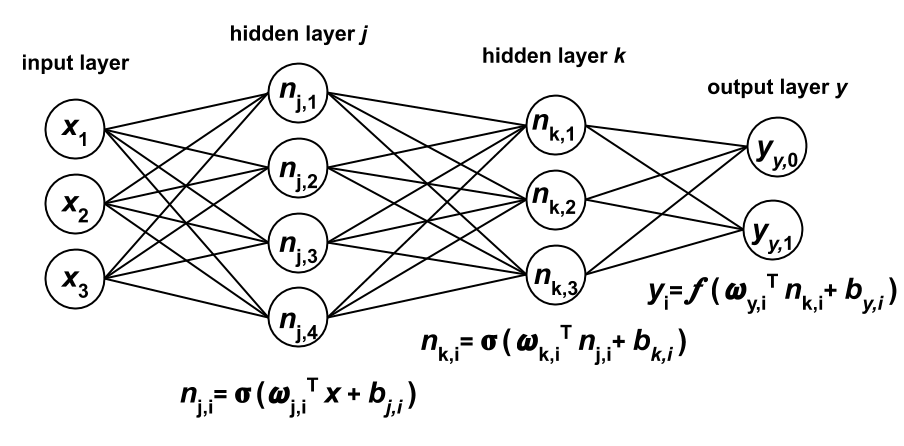
\includegraphics[width=\textwidth]{mlp}
    \caption{A feedforward network where on each neuron there is a label representing the value computed by it and passed to the nodes of the next layer through the arcs connecting them. A neuron assigns a weight $ \omega $ to each incoming arch and performs the shown linear combination. The sigmoid funciton of equation (\ref{eq:sigmoid}) can be used as the activation function $\sigma$. The function computed by the neurons in the output layer could be $softmax$ (\ref{eq:softmax}) where $\vect{v}_i = \vect{\omega}_{y,i}^T\vect{n}_k + b_{y,i}$. Here the bias $ b $ is explicited in the computation rather than adding another dimension to the various vectors $ \vect{\omega} $, $ \vect{n}$, and $ \vect{x} $ so that $ \omega_{r,i,0} = b_{r,i} $ for $ r \in \{j,k,y\} $ and $ x_{0} = n_{p,0} = 1 $ for $p \in \{j,k\} $.}
\label{fig:mlp}
\end{figure}

Consider the pair $(\vect{x}, y)$ consisting of a data point and its corresponding label, let $\hat{{y}}$ be the label predicted by the network, in order to assest the goodness of the prediction a non-negative loss function $\ell(y,\hat{y})$ is used so that the greater is the value of the loss the worse is the prediciton. In the case of a classification problem $y \in Y$, where $Y$ is the ordered set of possible symbolic labels, and $|Y| = m$, therefore by having a network with $m$ neurons in the output layer and using the $softmax$ function, the network prediction $\vect{\hat{y}}$ represents a probability distribution over $Y$ given the data point $\vect{x}$. For conveniency of notation let $y^*_i$ indicate the first element of $Y$ for $i = 0$, the second element of $Y$ for $i = 1$ and so on for all the elements of $Y$. This means that the $i$-th element of $\vect{\hat{y}}$ gives the probability that the label for data point $\vect{x}$ will be $y^*_i$ in the network prediction. In this case as the loss function the categorical cross-entropy loss can be used and it is defined as:
\begin{equation}
\label{eq:cross-entropy}
\ell(y,\hat{y}) = -\sum_{i=0}^{m-1}{\mathbb{I}(y^*_i = y)\log(\hat{y_i})} 
\end{equation}
where $\mathbb{I}(E) \in \{0, 1\}$ is the indicator function of an event $E$, meaning that $\mathbb{I}(E) = 1$ if and only if $E$ occours and $\mathbb{I}(E) = 0$ otherwise. Equation \ref{eq:cross-entropy} can be simplified to
$$
\ell(y, \hat{y}) = -log(\hat{y_i}) \text{, where } i \text{ verifies } y^*_i = y
$$

%explain how to optimize with backpropagation
%talk about using relu rather than sigmoid
%introduce cnn (read book on what to write)
%introduce regularization tecniques such as dropout, l2reg, batchNorm



\section*{The Street View House Number dataset}

\section*{Model training}

\section*{Results}



\end{document}




















